%\documentclass{cumcmthesis}
\documentclass[withoutpreface,bwprint]{cumcmthesis} %去掉封面与编号页,电子版提交的时候使用。


\usepackage[framemethod=TikZ]{mdframed}
\usepackage{url}   % 网页链接
\usepackage{subcaption} % 子标题
\title{全国大学生数学建模竞赛编写的 \LaTeX{} 模板}
\tihao{A}
\baominghao{xxxx}
\schoolname{XX大学}
\membera{ }
\memberb{ }
\memberc{ }
\supervisor{ }
\yearinput{2023}
\monthinput{09}
\dayinput{04}

\begin{document}

 \maketitle
 \begin{abstract}
国赛加油

\keywords{\TeX{}\quad  图片\quad   表格\quad  公式}
\end{abstract}

%目录  2019 明确不要目录,我觉得这个规定太好了
%\tableofcontents




\section{问题背景及重述}
\subsection{问题背景}
无创产前技术(NITP)利用新一代测序技术对孕妇外周血中的胎儿游离DNA进行检测,能够有效筛查唐氏综合征(21-三体综合征)、爱德华氏综合征(18-三体综合征)和帕陶氏综合征(13-三体综合征)三大染色体疾病,确定胎儿的健康状况。相比羊水穿刺和绒毛活检等传统产前诊断方法,NIPT技术无需进行侵入性操作,大大降低了因侵入性操作导致的流产、感染等风险,为高龄或有流产风险的孕妇提供了一种安全的替代方案。
\par 然而,NIPT的准确性受到孕妇的孕周数、胎儿性别、胎儿性染色体浓度等多种因素的影响。研究表明,男胎Y染色体浓度与孕妇的孕周数和BMI紧密相关。因此,合理选择NIPT的检测时点对于提高检测的准确性和减少潜在风险至关重要。此外,实际检测中还可能出现测序失败的情况,这进一步增加了检测的复杂性和不确定性。

\subsection{问题重述}
附件给出了某地区孕妇的NIPT数据,为了优化NIPT的检测策略,提高检测的准确性和可靠性,需要对NIPT的检测时点和胎儿异常判定方法进行深入研究。
\par 问题一:分析胎儿 Y 染色体浓度与孕妇的孕周数和 BMI 等指标的相关特性,建立相应的关系模型,并检验其显著性。
\par 问题二:临床证明,男胎孕妇的BMI是影响胎儿Y染色体浓度的最早达标时间(即浓度达到或超过4\%的最早时间)的主要因素。对男胎孕妇的BMI进行合理分组,给出每组的BMI区间和最佳NIPT时点,使得孕妇可能的潜在风险最小,并分析检测误差对结果的影响。 
\par 问题三:男胎的Y染色体浓度达标时间受到身高、体重、年龄等多种因素影响,综合考虑这些因素、检测误差和胎儿的 Y 染色体浓度达标比例(即浓度达到或超过 4\%的比例),根据男胎孕妇的BMI,给出合理分组以及每组的最佳NIPT时点,使得孕妇潜在风险最小,并分析检测误差对结果的影响。 
\par 问题四:由于孕妇和女胎都不携带 Y 染色体,以上方法无法判定女胎是否异常。以女胎孕妇的21号、18号和13号染色体非整倍体为判定结果,综合考虑X染色体及上述染色体的 Z值、GC含量、读段数及相关比例、BMI等因素,给出女胎异常的判定方法。


\section{模型假设}
\begin{enumerate}
    \item 假设孕周数与NIPT检测风险在三个不同风险区间上存在分段线性关系。
    \item two
    \item ...
\end{enumerate}


\section{符号说明}
\begin{table}[H]
\centering
\begin{tabular}{>{\hspace{0pt}}m{0.163\linewidth}>{\hspace{0pt}}m{0.592\linewidth}>{\hspace{0pt}}m{0.148\linewidth}} 
\hline
\multicolumn{1}{>{\centering\hspace{0pt}}m{0.163\linewidth}}{符号} & \multicolumn{1}{>{\centering\hspace{0pt}}m{0.592\linewidth}}{含义} & \multicolumn{1}{>{\centering\arraybackslash\hspace{0pt}}m{0.148\linewidth}}{单位}  \\ 
\hline
Y                                                                & 胎儿Y染色体浓度                                                         & 无量纲                                                                              \\
BMI                                                              & 孕妇的身体质量指数                                                        &                                                                                  \\
GW                                                               & 检测孕周数                                                            & 周                                                                                \\
T min                                                            & 胎儿Y染色体浓度首次达标时间                                                   & 周                                                                                \\
T k                                                              & 第k组的最佳NIPT时点                                                     & 周                                                                                \\
R k.mis                                                          & 误差函数                                                             &                                                                                  \\
R k.risk                                                         & 风险函数                                                             &                                                                                  \\
R k                                                              & 总风险函数                                                            &                                                                                  \\
\hline
\end{tabular}
\end{table}

%根据要求,电子版论文提交时需去掉封面和编号页。可以加上 \verb|withoutpreface|  选项来实现,即:
%\begin{tcode}
%    \documentclass[withoutpreface]{cumcmthesis}
%\end{tcode}
%这样就能实现了。打印的时候有超链接的地方不需要彩色,可以加上 \verb|bwprint| 选项。

%另外目录也是不需要的,将 \verb|\tableofcontents| 注释或删除,目录就不会出现了。

%团队的信息填入指定的位置,并且确保信息的正确性,以免因此白忙一场。

%编译记得使用 \verb|xelatex|,而不是用 \verb|pdflatex|。在命令行编译的可以按如下方式编译:
%\begin{tcode}
%	xelatex example
%\end{tcode}
%或者使用 \verb|latexmk| 来编译,更推荐这种方式。
%\begin{tcode}
%	latexmk -xelatex example
%\end{tcode}
%下面给出写作与排版上的一些建议。























\section{问题一的建模与求解}
\subsection{问题分析}
问题一的核心在于探究男胎Y染色体浓度与孕妇孕周数及身体质量指数(BMI)之间的相关性。
既往研究表明,男胎Y染色体浓度与孕妇孕周数和BMI存在紧密关联。
根据Zhou等人(2015)的研究,男胎Y染色体浓度与孕妇BMI呈负相关关系。
利用附件中的数据,我们对男胎Y染色体浓度与孕周数和BMI的相关性进行分析,
并构建回归模型拟合数据。
\subsection{数据预处理}
附件表格中给到的孕周数为周和日的混合单位,我们首先将该数据的单位统一转化为周,
不满一周的用小数表示。\par
GC含量是测序数据质量 评估中的一个重要指标,GC含量过高、过低、
或分布异常可能意味着测序质量存在问题。而对于男胎的Y染色体浓度,若该值小于4\%,
则NIPT的结果准确性较低。我们绘制了这两项数据的箱线图,直观展示数据的集中趋势、
分散程度和偏态,并剔除了36份异常值。
\begin{figure}[!h]
    \centering
    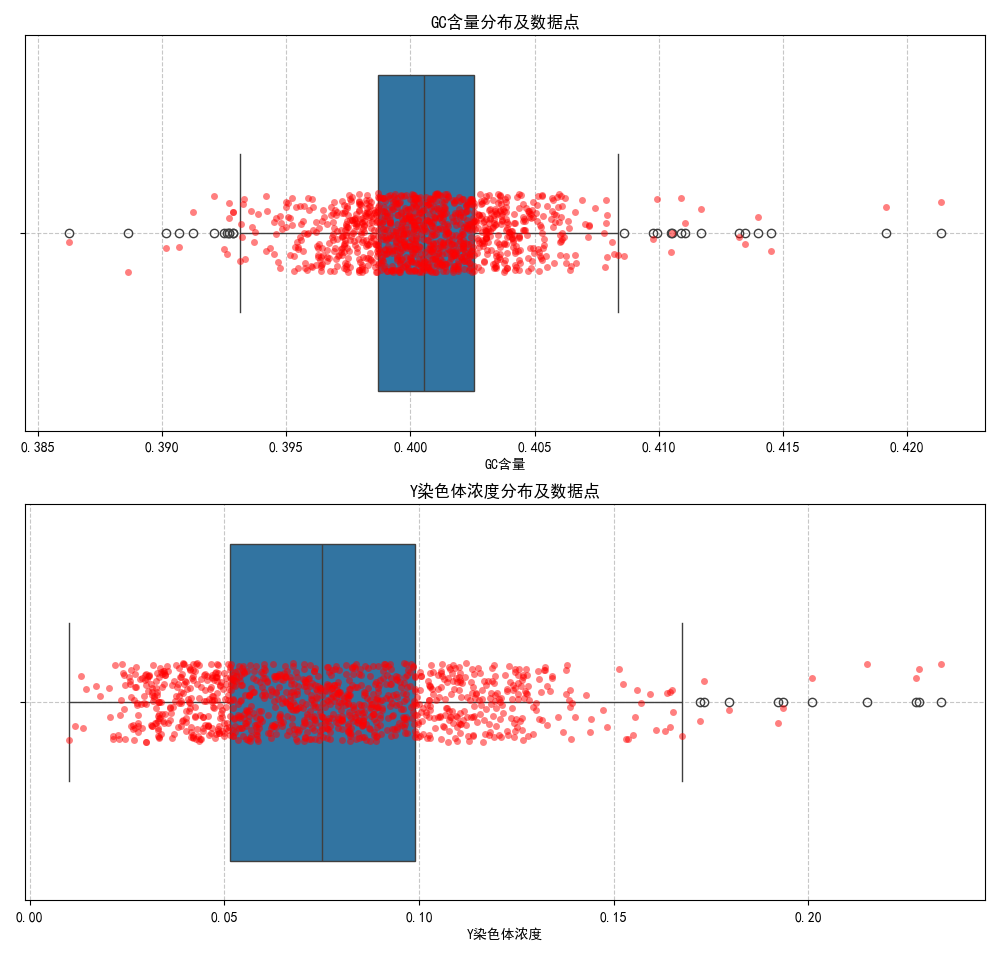
\includegraphics[width=1\textwidth]{箱线图.png}
    \caption{箱线图}
    \label{fig1}
\end{figure}

\subsection{正态分布检验}
为了判断使用皮尔逊相关性分析还是斯皮尔曼相关性分析,
我们首先检验了孕妇BMI,孕周数和Y染色体浓度数据的分布情况,
通过计算$p$值判断数据是否符合正态分布。在统计学中,
Kolmogorov-Smirnov(K-S)检验是一种非参数检验方法,
适用于检验数据是否服从某一特定分布,如正态分布。我们采用K-S检验,
计算数据的累积分布函数与理论分布的累积分布函数之间的最大差异,并据此计算$p$值。
\par 假设理论分布为正态分布,理论分布的累积分布函数
$$
F_{\left( x \right)}=\varPhi \left( \frac{x-\mu}{\sigma} \right) 
$$
其中,$\varPhi$是标准正态分布的累积分布函数,$\mu$为均值,$sigma$为标准差。
对样本数据$X=\left\{ x_1,x_2,...,x_n \right\}$进行排序,得到排序后的数据
$X_{store}=\left\{ x_{\left( 1 \right)},x_{\left( 2 \right)},...,x_{\left( n \right)} \right\} $。
对于排序后的数据点$x_{\left( 1 \right)}$,计算其经验累积分布函数(CDF)
$$
F_i=\frac{i}{n}
$$
其中,$i$是数据点的排名,$n$是样本量。\par
对于每个排序后的数据点$x_{(i)}$,计算理论分布的累积分布函数(理论CDF)
$$
F(x_{(i)}) = \Phi \left( \frac{x_{(i)} - \mu}{\sigma} \right)
$$
再计算样本CDF与理论CDF之间的最大绝对差异$D$:
$$
D = \max_{1 \leq i \leq n} \left| F_i - F(x_{(i)}) \right|
$$
通过K-S分布来计算$p$的值,K-S统计量$D$的分布可以近似为:
$$
p \approx Q(\sqrt{n}D)
$$
其中$Q$为K-S分布的累积分布函数的补数:
$$
Q(x) = 2 \sum_{k=1}^{\infty} (-1)^{k-1} e^{-2k^2x^2}
$$
最终通过$p$值相对于显著水平的大小判断样本是否符合正态分布
$$
\left\{ \begin{array}{l}
	p>0.05\text{,服从正态分布}\\
	p<0.05\text{,不服从正态分布}\\
\end{array} \right. 
$$

我们计算出这三个变量的$p$值,同时还分别绘制了样本的分布直方图,
发现所有数据都不符合正态分布,因此选择斯皮尔曼相关系数用于评估变量之间的相关特性。
\begin{table}[!h]
\caption{p值计算结果}\label{tab:1}
\centering
\begin{tabular}{>{\centering\hspace{0pt}}m{0.292\linewidth}>{\centering\hspace{0pt}}m{0.275\linewidth}>{\centering\arraybackslash\hspace{0pt}}m{0.337\linewidth}} 
\toprule
特征     & p值          & 结论       \\ 
\hline
检测孕周数值 & 2.37448E-22 & 不符合正态分布  \\
孕妇BMI  & 1.41177E-19 & 不符合正态分布  \\
Y染色体浓度 & 1.48E-14    & 不符合正态分布  \\
\bottomrule
\end{tabular}
\end{table}

\subsection{斯皮尔曼相关性分析}
斯皮尔曼秩相关系数用$r_s$表示,是一种非参数统计方法,
用于评估两个变量之间的单调关系。对比皮尔逊相关系数,
斯皮尔曼相关系数不依赖于数据的分布,而是根据数据的秩来计算,
使得它对异常值和非正态分布的数据更为鲁棒。先对两个变量的数据分别进行排序,
得到每个数据点的秩。然后对于每一对数据点,计算秩的差值,计算出斯皮尔曼系数,
公式如下:
\begin{equation}\label{1}
r_s=1-\frac{6\sum{d_i^2}}{n\left( n^2-1 \right)}
\end{equation}
其中$d_i$是两个变量的秩的差值,$n$是数据点的数量。\par
$r_s\in[-1,1]$,
且$\left| r_s \right|$越接近1,相关性越强。若斯皮尔曼相关系数$r_s<0$,
认为两个变量之间存在正相关,如果$r_s=1$,则说明两组变量呈完全正相关性;
反之,若斯皮尔曼相关系数$r_s<0$,则认为两个变量之间存在负相关,
如果$r_s=-1$,则两组变量呈完全负相关性。\par
按照此方法,我们分别计算出各个可能影响因素和男胎Y染色体浓度之间的相关性,
并用热力图表示,结果如下:
\begin{figure}[!h]
    \centering
    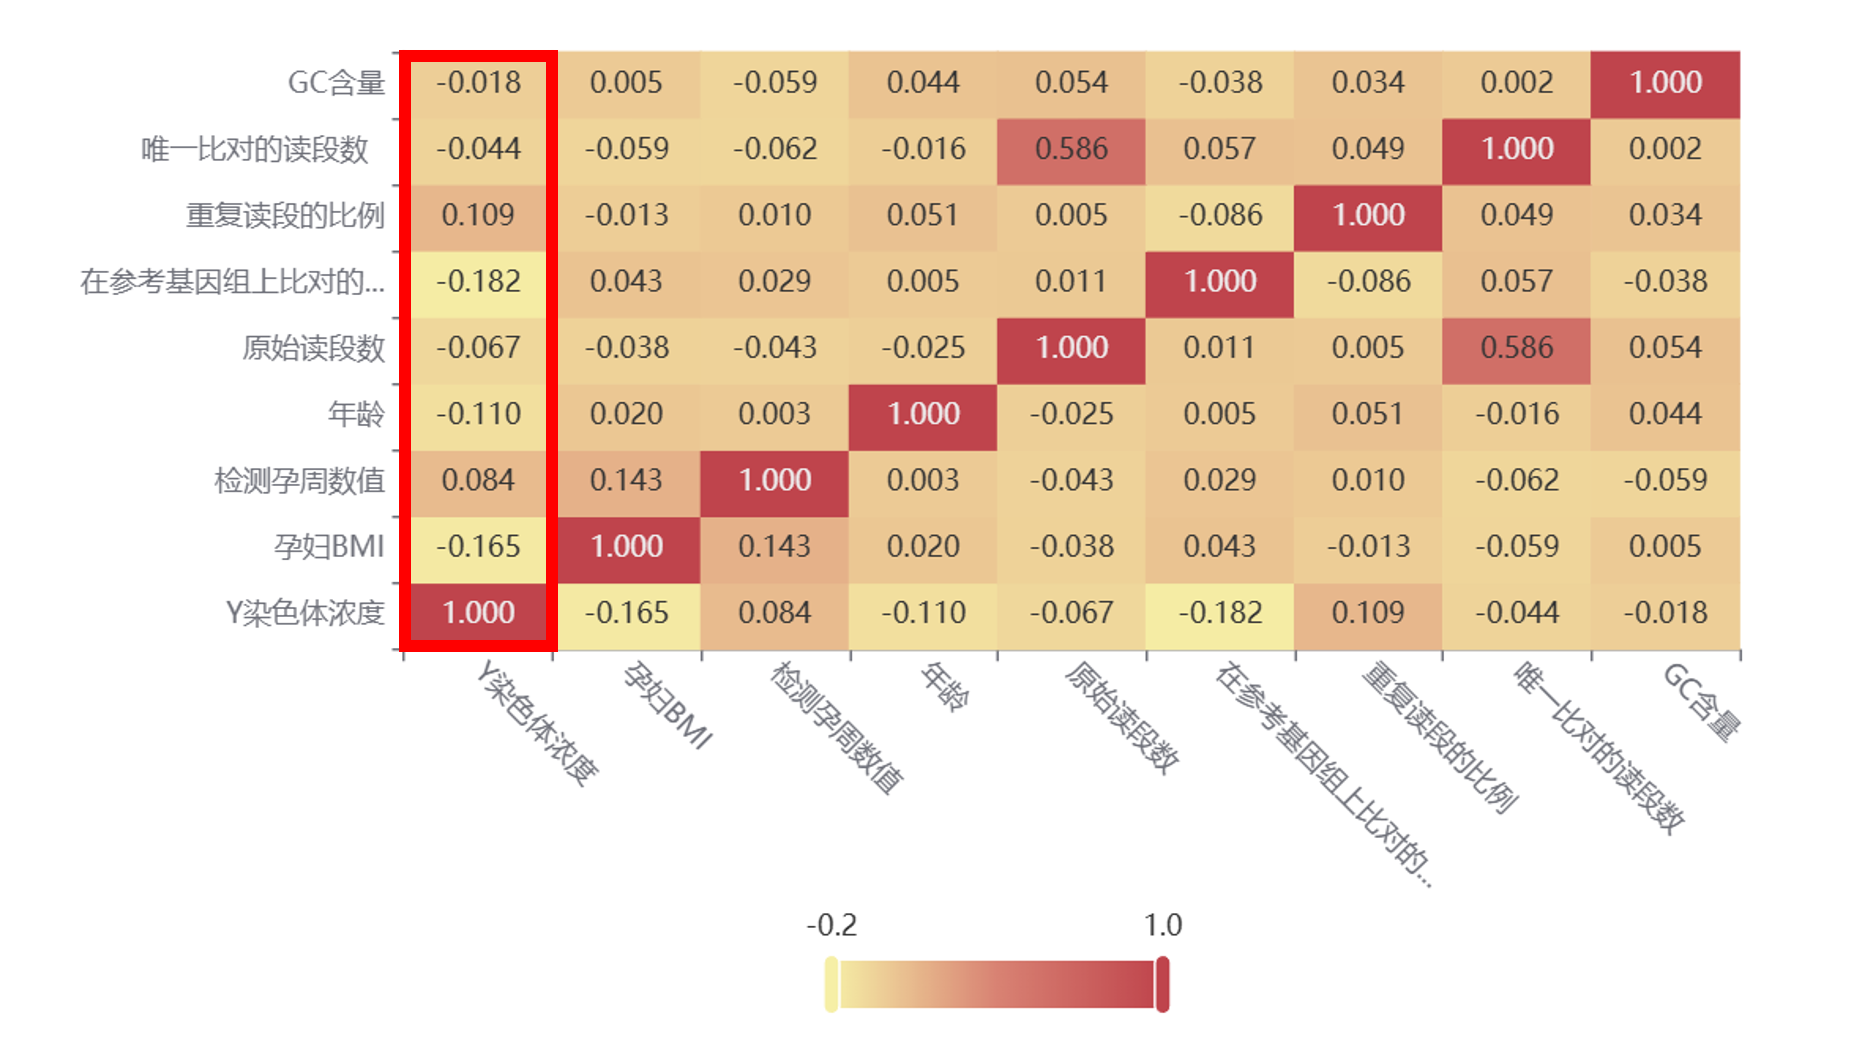
\includegraphics[width=1\textwidth]{斯皮尔曼相关系数热力图.png}
    \caption{斯皮尔曼相关系数}
    \label{fig4}
\end{figure}

\subsection{建立回归模型}
观察到孕妇BMI、孕周数和男胎Y染色体浓度之间的关系,我们尝试对其构建回归模型。
我们首先采用了简单的多元线性回归:
\begin{equation}\label{2}
Y_i=\alpha _0+\beta _1\cdot BMI_i+\beta _2\cdot GW_i+\epsilon_i 
\end{equation}
其中$\beta _0$,$\beta _1$,$\beta _2$为模型的固定效应参数,分别代表截距、
BMI的系数、以及孕周数的系数。$\epsilon_i$为服从正态分布的随机误差项,
$\epsilon _i~N\left( 0,\sigma ^2 \right) $。
但根据得到的结果,初步模型的拟合效果并不理想,
表现为较低的决定系数$R^2$值。\par
在多元线性回归的基础上,我们通过引入多项式特征转换,
将模型扩展为能够捕捉非线性关系的非线性模型:
\begin{equation}\label{3}
Y_i=\alpha _0+\sum_{m=1}^p{\beta}_m\cdot BMI_{i}^{m}+\sum_{n=1}^q{\gamma}_n\cdot GW_{i}^{n}+\epsilon _i
\end{equation}
考虑到数据具有层次结构,同一孕妇的数据会被多次测量,为了捕捉数据中的随机效应,
适应数据中的个体差异,我们结合前面模型的优点,构建非线性混合效应模型。
这种模型不仅包括固定效应,还包括随机效应,能够适应数据中的个体差异,
并有效处理数据中的随机变异性。
\begin{equation}
Y_{ij}=\alpha _0+\sum_{m=1}^p{\beta}_m\cdot BMI_{ij}^{m}+\sum_{n=1}^q{\gamma}_n\cdot GW_{ij}^{n}+b_{0j}+\epsilon _{ij}
\end{equation}
其中$Y_{ij}$为第$i$位孕妇第$j$次检测时男胎的Y染色体浓度,
$BMI_{ij}$,$GM{ij}$分别代表检测时的BMI和孕周数。
$b_{0j}$为随机效应,表示与第j次测量相关的随机效应系数(随机截距),
它捕捉了组内变异,也服从正态分布$N\left( 0,\sigma _b^2 \right)$,
$\sigma _b^2$为随机效应的方差。


\subsection{模型结果}
在得到模型之后,我们通过改变p和q的值来拟合不同次数的多项式模型。
为了选择最佳的模型,我们使用了赤池信息准则(AIC)作为模型选择的标准。
AIC是一种衡量统计模型相对质量的准则,它考虑了模型的拟合优度和模型的复杂程度,
值越小代表模型越好。
$$
AIC=2k-2\ln \left( \hat{L} \right) 
$$
其中,$k$是模型的参数数量(包括截距项),$\hat{L}$是模型的最大似然估计。\par
我们对每一对$p$和$q$的组合进行了模型拟合,并计算出相应的AIC值。此外,
我们检查了每个模型参数的$P$值,以确定其统计显著性。经过比较,我们发现当$p=4$和$q=3$时,
模型的AIC值最小,既能很好地拟合数据,又不会过于复杂。
同时该模型的决定系数$R^2$达到了0.80558,表明模型能解释大部分的变异。
据此我们最终的模型如下:
\begin{equation}\label{3}
Y_{ij}=\alpha _0+\sum_{m=1}^4{\beta}_m\cdot BMI_{ij}^{m}+\sum_{n=1}^3{\gamma}_n\cdot GW_{ij}^{n}+b_{0j}+\epsilon _{ij}
\end{equation}


\begin{table}
\caption{模型系数具体取值}\label{tab:2}
\centering
\begin{tabular}{|>{\hspace{0pt}}m{0.285\linewidth}|>{\hspace{0pt}}m{0.15\linewidth}|>{\hspace{0pt}}m{0.2\linewidth}|>{\hspace{0pt}}m{0.242\linewidth}|} 
\hline
\multicolumn{1}{|>{\centering\hspace{0pt}}m{0.285\linewidth}|}{变量名称} & \multicolumn{1}{>{\centering\hspace{0pt}}m{0.15\linewidth}|}{模型系数} & \multicolumn{1}{>{\centering\hspace{0pt}}m{0.2\linewidth}|}{估计值} & \multicolumn{1}{>{\centering\arraybackslash\hspace{0pt}}m{0.242\linewidth}|}{显著性水平(p值)}  \\ 
\hline
固定效应截距                                                                 & $\alpha _0$                                                                   & -41.2744                                                           & 0.002021                                                                          \\ 
\hline
$BMI$                                                              & $\beta _1$                                                                   & 5.0546                                                             & 0.001954                                                                          \\ 
\hline
$BMI^2$                                                             & $\beta _2$                                                                   & -0.2317                                                            & 0.001860                                                                          \\ 
\hline
$BMI^3$                                                              & $\beta _3$                                                                   & 0.0047                                                             & 0.001783                                                                          \\ 
\hline
$BMI^4$                                                              & $\beta _4$                                                                   & -3.56E-05                                                          & 0.001717                                                                          \\ 
\hline
$GM$                                                              & $\gamma _1$                                                                   & 0.0289                                                             & 0.000676                                                                          \\ 
\hline
$GM^2$                                                               & $\gamma _2$                                                                   & -0.0016                                                            & 0.000848                                                                          \\ 
\hline
$GM^3$                                                               & $\gamma _3$                                                                   & 3.13E-05                                                           & 0.000317                                                                          \\ 
\hline
随机效应截距                                                               & $b_{0j}$                                                                   & 2.9421                                                             & 5.30E-18                                                                          \\
\hline
\end{tabular}
\end{table}


\newpage
\section{问题二的建模与求解}
\subsection{问题分析}
在问题一中我们找到了Y染色体浓度与孕妇BMI和孕周数之间的非线性关系,
而问题二需要我们对孕妇的BMI进行合理分组并判断最佳NIPT检测时点,
以最小化因胎儿异常导致的潜在风险及误差对结果的影响。若检测时间过早,
男胎的Y染色体浓度未达4\%,NIPT检测结果准确性较低;若检测时间过晚,
则会带来治疗窗口期缩短的风险。
已知胎儿Y染色体浓度达到或超过4\%的最早时间主要受到孕妇BMI的影响。
我们将孕妇的BMI分为k组,并对NIPT检测的总风险$R_s$进行量化,
通过使总风险最小求出每组对应的最佳检测时点$T_k$。

\subsection{量化误差}
我们将误差定义为在特定检测时间点$T_k$,胎儿Y染色体浓度未达到4\%值的概率。
这可能会导致NIPT检测结果错误,增加治疗窗口期风险。
由于孕周数$GM$和检测节点$T_k$均指代同一概念,即截至检测时点孕妇的怀孕时长。
为了避免混淆并保持术语的一致性,后续讨论将统一使用$T_k$来指代这一指标。
通过问题一的结论,我们得到在特定检测时点下的胎儿Y染色体浓度
$f\left( T_k,BMI \right)$,并定义误差为
\begin{equation}
R_{k\cdot mis}=P\left( f\left( T_k,\text{BMI} \right) <4\% \right) =\Phi \left( \frac{4\%-f\left( T_k,\text{BMI} \right)}{\sqrt{\sigma _b^2}} \right) 
\end{equation}
其中$\varPhi$为标准正态累积分布函数,$\sigma _b^2$为随机效应的方差。\par
该误差会随着时间而变化。若检测太早($T_k$太小),$f\left( T_k,BMI \right)$
可能未上升至4\%,误差高;若检测太晚($T_k$太大),浓度可能已达标,因为测量噪声,、
该误差仍然存在。BMI分组会影响f$f\left( T_k,BMI \right)$的轨迹,
进而影响误差曲线。

\subsection{量化风险}
我们将风险定义为由于检测时间选择不当(即超过孕28周)
而导致治疗窗口期缩短的潜在危害。根据临床研究,
我们发现风险水平随着孕周的增加而变化,具体表现为:
早期阶段(孕周小于12周)风险相对较低,有足够的时间进行干预和治疗;
中期阶段(孕周在13至27周之间)风险逐渐升高,治疗的紧迫性也随之增加;
晚期阶段(孕周超过28周)风险极高,治疗窗口期已经大幅缩短,
干预措施的难度和复杂性显著增加。风险随检测时间延迟于“最佳检测时间”而增加,
这一现象在临床实践中得到了广泛证实。为了量化这一风险,
我们假设在这三个风险检测的不同区间内,风险与时间之间存在线性关系,
并通过一个分段线性函数来表示风险随时间的变化
\begin{equation}
R_{k\cdot risk}=\left\{ \begin{array}{l}
	c_1\cdot T_k\ \ \ \ \ \ \ \ \ \ \ \ \ \ \ \ \ \ \ \ \ \ \ \ \ \ \ \ \ \ \ \ \ \ \ \ \ \ \ \ \text{当}T_k<12\ \text{(早期阶段)}\\
	12c_1+c_2\cdot \left( T_k-12 \right) \ \ \ \ \ \ \ \ \ \ \ \ \ \ \ \ \text{当}13<T_k<27\ \text{(中期阶段)}\\
	12c_1+15c_2+c_3\cdot \left( T_k-21 \right) \ \ \ \ \text{当}T_k>28\ \text{(晚期阶段)}\\
\end{array} \right.   
\end{equation}
其中$c_1$,$c_2$,$c_3$是权重系数,我们先对这三个系数进行初始赋值,
再基于历史数据进行不断校准。\par
定义$T_{min}$为Y染色体浓度首次达到4\%的时间
,及最理想的检测点。根据问题一的模型可以对$T_{min}$求解:
$$
T_{min}=\min \left\{ T_k|f\left( T_k,BMI \right) \ge 0 \right\} 
$$
风险在$T_k=T_{min}$时最小,之后随延迟指数增长。BMI分组会影响$T_{min}$,
从而影响风险曲线。

\subsection{构建总风险函数}
误差$R_{k\cdot\text{mis}}$主要与Y染色体浓度低于所需阈值有关,
这可能导致NIPT结果的不准确,Y染色体浓度达到4\%是确保检测结果准确性的最低要求。
因此,$R_{k\cdot\text{mis}}$会推迟检测时间,拉高$T_k$。另一方面,
尽早通过检测发现不健康的胎儿对于降低治疗窗口期缩短的风险至关重要。
这意味着尽管推迟检测可能减少检测误差,但它同时增加了健康风险。
因此,$R_{k\cdot\text{risk}}$倾向于促使检测时间提前,降低$T_k$。
综合考虑误差和风险,我们需要为这两个因素分配适当的权重,
并构造一个总风险函数$R_k$来描述在孕周$T_k$进行NIPT的总风险:
$$
R_k = w_{\text{mis}} \cdot R_{k\cdot\text{mis}} + w_{\text{risk}} \cdot R_{k\cdot\text{risk}}
$$
其中,$w_{mis}$和$w_{risk}$分别是检测误差和健康风险的权重,
反映不同风险因素在决策过程中的重要性。为了简化模型,我们另权重的加和为1,得到:
\begin{equation}
R_k=\lambda \cdot R_{k\cdot \text{mis}}+\left( 1-\lambda \right) \cdot R_{k\cdot \text{risk}}
\end{equation}
\par 在得到第k组所对应的NIPT总风险$R_s$后,将各组的总风险函数加和,
并对该目标函数进行求最小资值。
$$
\sum_{k=1}^k{P\left( BMI\epsilon \left( b_{k-1},b_k \right) \right) \cdot R_k}
$$
我们基于L-BFGS算法对模型进行优化,因为它适用于大规模问题,且能够有效处理有界约束。
L-BFGS算法通过近似计算Hessian矩阵的逆来寻找函数的局部最小值,
而不需要存储整个矩阵,从而显著减少了内存需求。
在优化过程中通过反复调整参数,我们得出当$k=4$时,能保证目标函数的和最小。据此,
我们得到最终分组结果,以及每组相应的最佳NIPT时点,结果如下:

\begin{table}[H]
\caption{BMI分组及最佳NIPT时点}
\centering
\begin{tabular}{>{\centering\hspace{0pt}}m{0.129\linewidth}>{\centering\hspace{0pt}}m{0.406\linewidth}>{\centering\arraybackslash\hspace{0pt}}m{0.348\linewidth}} 
\hline\hline
组别 & 孕妇BMI区间       & 最佳NIPT时点  \\ 
\hline
1  & (27.1,30.16]  & 11        \\
2  & (30.16,31.74] & 12        \\
3  & (31.74,33.78] & 12.3      \\
4  & (33.78,39.1]  & 23.3      \\
\hline\hline
\end{tabular}
\end{table}

\subsection{误差分析}
为了分析测量误差的影响,我们对模型进行了灵敏度分析,
通过改变随机效应的标准差$\sigma _b$模拟不同的测量误差水平。
对于每个BMI组,我们重新计算了总风险$R_k$和最佳NIPT时点$T_k$,
同时计算了相应的损失。从结果分析,损失值在$\sigma _b$变化时基本保持稳定,
大约在0.5左右。这表明模型对于测量误差的变化具有较好的鲁棒性,
即测量误差的增加并没有显著影响模型的损失。
\begin{figure}[!h]
    \centering
    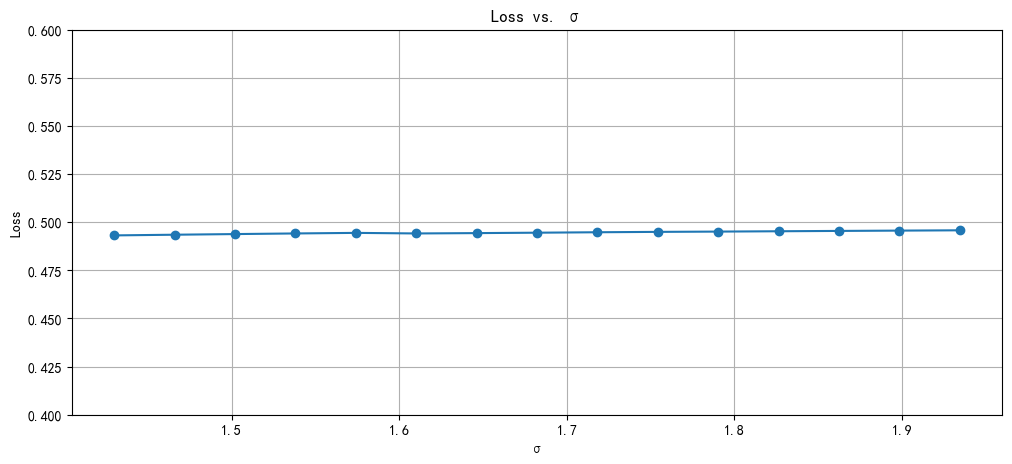
\includegraphics[width=1\textwidth]{损失&标准差.png}
    \caption{测量误差对模型损失的影响}
    \label{fig5}
\end{figure}
\par 而对于$T_k$,不同组别的最优检测时间对测量误差的敏感性不同。
前三组的最优检测时间不受测量误差的影响,
而第四组的最优检测时间在一定程度上受测量误差的影响,
这可能与第四组的检测窗口期较短有关。
\begin{figure}[!h]
    \centering
    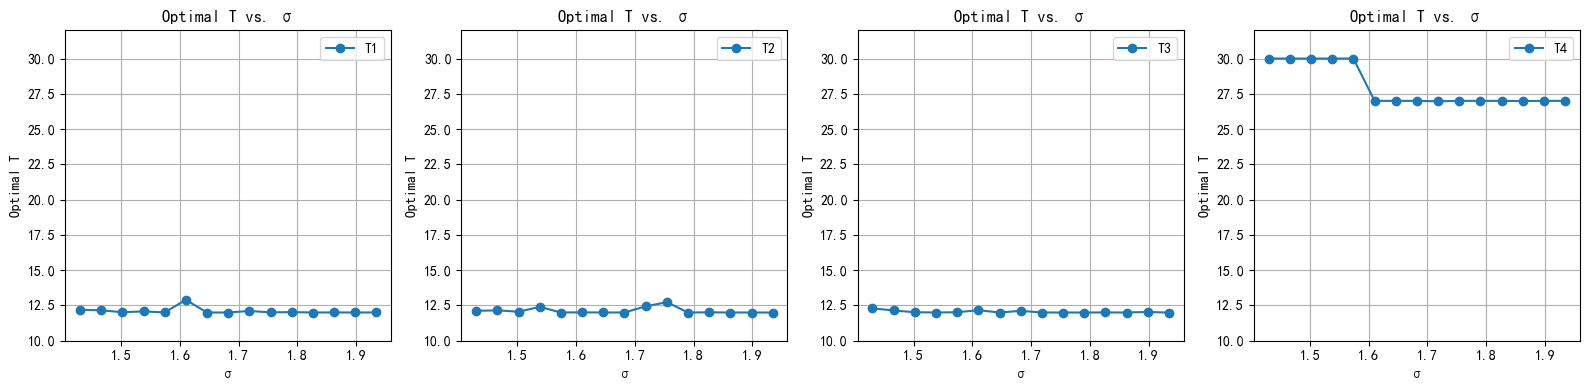
\includegraphics[width=1\textwidth]{T&标准差.png}
    \caption{测量误差对最优检测时间的影响}
    \label{fig6}
\end{figure}


\section{问题三的建模与求解}
\subsection{问题分析}











%参考文献
\begin{thebibliography}{9}%宽度9
    \bibitem[1]{1}
    施炜慧,徐晨明. 无创产前检测在产科母体并发症和合并症诊断中的应用价值 [J].实用妇产科杂志,2025,41(08):617-620.
    \bibitem[2]{2}
    吴军,崔云静,郭飞波,等.BMI与IVF/ICSI-ET术后自然流产胚胎染色体核型异常的关系[J].河北医学,2021,27(08):1279-1284.
    \bibitem[3]{3}
    Zhou Y ,Zhu Z ,Gao Y , et al.Effects of Maternal and Fetal Characteristics on Cell-Free Fetal DNA Fraction in Maternal Plasma[J].Reproductive Sciences,2015,22(11):1429-1435. 
    \bibitem[4]{4}
    丁乐,韩峰,王稼琪,等.基于斯皮尔曼相关系数的高加快速减负荷分析及控制策略完善[J].能源工程,2025,45(03):16-20.
    \bibitem[5]{5}
    蓝志衡.DNA序列分布比率法在无创产前胎儿染色体非整倍体检测中的应用[D].华南理工大学,2020\.DOI:10.27151/d.cnki.ghnlu.2020.005132.

\end{thebibliography}

\newpage


















%附录
\begin{appendices}

\section{利用分布直方图进行正态性可视化判断}
\begin{figure}[!h]
    \centering
    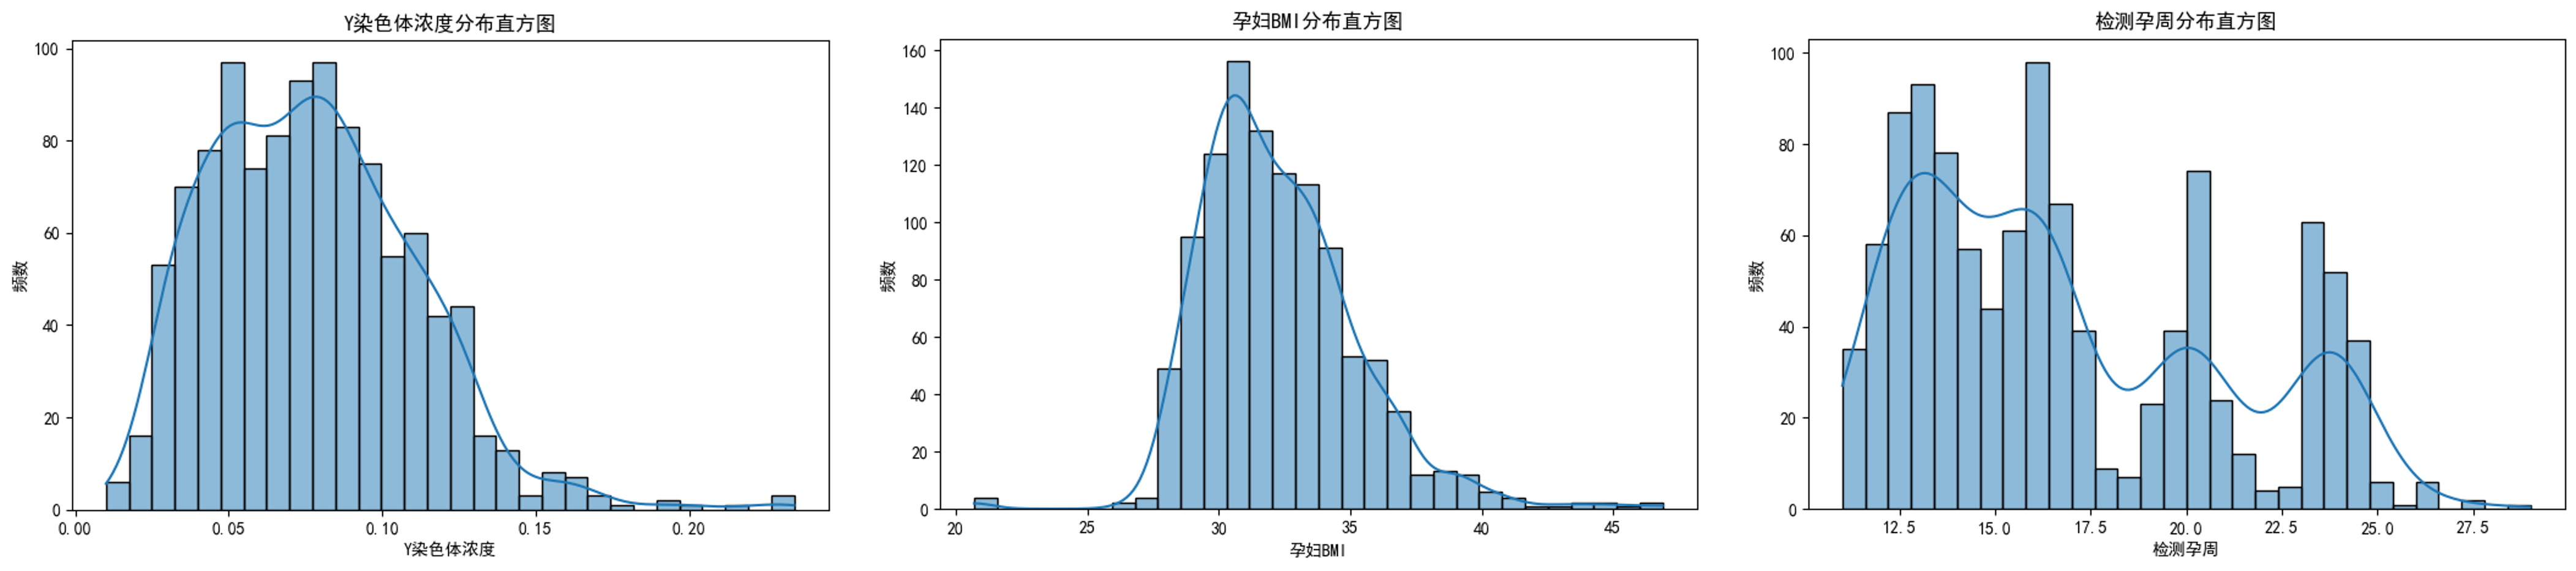
\includegraphics[width=1\textwidth]{分布直方图.png}
    \caption{Y染色体浓度、孕妇BMI、孕周数的分布直方图}
    \label{fig4}
\end{figure}

\section{非线性混合效应模型--python 源代码}

\begin{lstlisting}[language=python]
from scipy.stats import shapiro
import statsmodels.formula.api as smf
import statsmodels.api as sm
from  sklearn.metrics import r2_score, mean_squared_error
import json

p_list = [ i for i in range(1,6)]
q_list = [ i for i in range(1,6)]
results = {}
best_aic = np.inf

for p in p_list:
    for q in q_list:
        gw_terms = ' + '.join(f'I(检测孕周**{k})' for k in range(1, p+1))
        bmi_terms = ' + '.join(f'I(孕妇BMI**{k})' for k in range(1, q+1))

        formular = f'Y染色体浓度 ~ {gw_terms} + {bmi_terms}'

        mixed_model = smf.mixedlm(formula=formular, data=boy.data, groups=boy.data["孕妇代码"])
        result = mixed_model.fit()

        y = boy.data['Y染色体浓度']
        fitted = result.fittedvalues
        r2 = r2_score(y, fitted)
        mse = mean_squared_error(y,fitted)
        aic = 2 * result.llf + 2 * len(result.params)
        
        
        shapiro_stat, shapiro_p = shapiro(resid)
        normality = shapiro_p > 0.1

        log ={
            "r2": r2,
            "mse": mse,
            "shapiro_stat": shapiro_stat,
            "shapiro_p": shapiro_p,
            "normality": normality,
            "log-likelihood": result.llf,
            "aic": aic,
            "params": result.params.to_dict(),
            "pvalues": result.pvalues.to_dict()
        }
        results[f"p={p},q={q}"] = log

        if aic < best_aic:
            best_aic = aic
            results["best_model"] = log
    
with open("mixedlm_formulas_results.json", "w", encoding="utf-8") as f:
    json.dump(results, f, ensure_ascii=False, indent=2)
 \end{lstlisting}

 \section{规划解决程序--lingo源代码}

\begin{lstlisting}[language=c]
kk=2;
[mdd,ndd]=size(dd);
while ~isempty(V)
    [tmpd,j]=min(W(i,V));tmpj=V(j);
for k=2:ndd
    [tmp1,jj]=min(dd(1,k)+W(dd(2,k),V));
    tmp2=V(jj);tt(k-1,:)=[tmp1,tmp2,jj];
end
    tmp=[tmpd,tmpj,j;tt];[tmp3,tmp4]=min(tmp(:,1));
if tmp3==tmpd, ss(1:2,kk)=[i;tmp(tmp4,2)];
else,tmp5=find(ss(:,tmp4)~=0);tmp6=length(tmp5);
if dd(2,tmp4)==ss(tmp6,tmp4)
    ss(1:tmp6+1,kk)=[ss(tmp5,tmp4);tmp(tmp4,2)];
else, ss(1:3,kk)=[i;dd(2,tmp4);tmp(tmp4,2)];
end;
end
    dd=[dd,[tmp3;tmp(tmp4,2)]];V(tmp(tmp4,3))=[];
    [mdd,ndd]=size(dd);
    kk=kk+1;
end;
S=ss;
D=dd(1,:);
 \end{lstlisting}
\end{appendices}

\end{document} 